\documentclass{standalone}

\usepackage{pgfplots,tikz,amsmath}
\begin{document}
		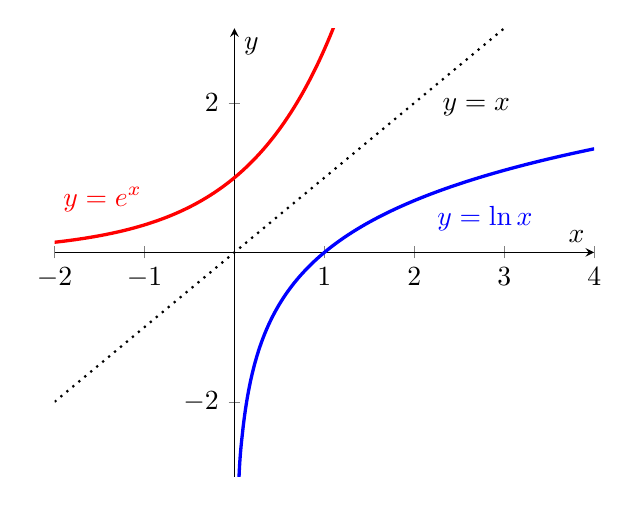
\begin{tikzpicture}[scale=1]             
			\begin{axis}[axis lines=center, xlabel={$x$}, ylabel={$y$}, domain=-2:4,
							ymin=-3, ymax=3,xmin=-2,xmax=4]
				\addplot[smooth, very thick, blue, samples=150] {ln(x)}
						[below right] node[pos=0.75] {\color{blue}$y=\ln{x}$};
				\addplot[smooth, very thick, red, samples=150] {exp(x)}
						[above left] node[pos=0.02] {\color{red}$y=e^{x}$};
				\addplot[smooth, black, dotted, thick] {x}
						[below right] node[pos=0.7] {\color{black}$y=x$};
			\end{axis}
		\end{tikzpicture}     
\end{document}
